%%%%%%%%%%%%%%%%%%%%%%%%%%%%%%%%%%%%%%%%%%%%%%%%%%%%%%%%%%%%%%%%%%%%%%%%%%%%%%%%%%%%%%%%%%%
%%%%%%%%%%%% Trabalho de final de curso em Eng. de Teleinformatica - UFC %%%%%%%%%%%%%%%%%%
%%%%%%%%%%%%%%%%%%%%%%%%%%%%%%%%%%%%%%%%%%%%%%%%%%%%%%%%%%%%%%%%%%%%%%%%%%%%%%%%%%%%%%%%%%%
%%%%%%%%%%%%%%%%%%%%%%%%%%%%%%%%%% Luiz Camara Neto %%%%%%%%%%%%%%%%%%%%%%%%%%%%%%%%%%%%%%%
%%%%%%%%%%%%%%%%%%%%%%%%%%%%%%%%%%%%%%%%%%%%%%%%%%%%%%%%%%%%%%%%%%%%%%%%%%%%%%%%%%%%%%%%%%%
%%%%%%%%%%%%%%%%%%%%%%%%%%%%%%% Metodos De Segmentacao %%%%%%%%%%%%%%%%%%%%%%%%%%%%%%%%%%%%
%%%%%%%%%%%%%%%%%%%%%%%%%%%%%%%%%%%%%%%%%%%%%%%%%%%%%%%%%%%%%%%%%%%%%%%%%%%%%%%%%%%%%%%%%%%

\chapter{Fundamentação Teórica}
\thispagestyle{empty}


\section{O Empreendedorismo}

Segundo o economista Joseph Schumpeter, o empreendedor é alguém versátil, que possui as habilidades técnicas para saber produzir, e capitalista, que consegue reunir recursos financeiros, organizar as operações internas e realizar as vendas da sua empresa \cite{Castor:2009}. A Global Entrepreneurship Monitor (GEM) 2015. Apoiado pelo Sebrae, e o estudo realizado pelo Instituto Brasileiro de Qualidade e Produtividade (IBQP), detectou que o Brasil atingiu nos dois últimos anos uma das maiores taxa de empreendedorismo inicial de sua história \cite{EmpreenderBrasil}.

Empreender em casa tem sido uma das formas mais comuns e mais baratas para se começar um negócio de venda de doces em casa ou nas ruas. Em 1988 o empresário Alexandre Tadeu da Costa, dono da confeitaria Cacau Show, com 18 anos colocava trufas e bombons de chocolate no banco de trás do carro e os vendia em padarias e supermercados da Zona Oeste de São Paulo (SP), hoje conta com mais de mil lojas em todo o país \cite{negociodozero}. 

O Sebrae dar as melhores orientações de como abrir um negócio na área de chocolates, trufas e bombons, o principais investimentos são: na estrutura (instalação da área de produção), compra e venda, legislação, planejamento, divulgação e gestão \cite{sebraenegociodoces}. 

A tecnologia hoje pode proporcionar para os negócios que estão começando, facilidades no controle de gestão financeira, gestão operacional, divulgação de trabalhos com marketing, analise de resultados, fidelização de clientes e ajudar na tomada de decisões ao planejar estratégias de melhoria contínua.


\section{A Web Moderna}\label{sec:web-moderna}

A Web tem mudado muito nos últimos anos, a web antiga, conhecida na década de 90, onde haviam páginas estáticas somente com o conteúdo de textos e imagens e com pouca interação foi evoluindo com a chegada de tecnologias no ano de 2000, como o Flash por exemplo, começava a ser mais comum ver animações e vídeos na web.Segundo (\citeautor{Marcondes}, \citeyear{Marcondes}), a chamada Web moderna ou web 2.0 faz muito uso de tecnologias como Javascript, transferência de dados(Ajax e WebSockets) e aplicações interativas. A Web hoje usa tecnologias como o Html5, comunicação assíncrona entre o cliente e servidor, utiliza técnicas de Single Page Application(SPA) e navegação sem links tradicionais.


\section{Arquitetura de Software}\label{sec:arquitetura}
“A arquitetura de software de um programa ou de um sistema computacional é a estrutura ou as estruturas do sistema, que compreende elementos de software, as propriedades visíveis e externas desses elementos, e as relações entre eles.”\cite{BASS}

\subsection{Arquitetura Tradicional}

No desenvolvimento de aplicações Web de hoje, ainda é muito utilizado um modelo onde um cliente(navegador), faz uma Solicitação  ao um servidor web, que contém código escrito em Python, Java, Php ou qualquer outra linguagem e executa uma série de tarefas, como processar dados vindos da Solicitação, regras de negócio, persistência ou recuperação de dados.Neste cenário, a lógica de negócio e de apresentação fica toda no servidor.Um exemplo comum seria um cliente solicitar uma página para realizar um cadastro de produto, é feito uma Solicitação ao servidor, o mesmo encontra a página executa algum processamento e envia texto para o cliente(navegador), após o preenchimento do formulário é feito o envio novamente para o servidor que obtém os dados do formulário, valida as informações e persistir no banco de dados ou invalida o processo e depois responde ao cliente.Veja uma ilustração abaixo de como seria este modelo:

\begin{figure}[!h]
\centering
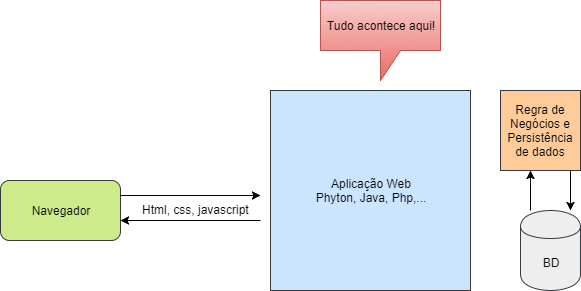
\includegraphics[width=8cm]{Figuras/Cap1/arquitetura-tradicional.png}
\caption[]{Figura mostra um Diagrama de uma arquitetura tradicional de desenvolvimento de aplicações we} 
\end{figure}

\subsection{Arquitetura Moderna}
Com o avanço de tecnologias como o Html 5, os negagadores e os frameworks no lado do cliente, surgiram novos modelos de arquiteturas para projetos de software, um deles e foi escolhido para desenvolver o sistema foi o SOFEA(Service Oriented Front-End Architecture), que é uma arquitetura para o Front-End orientada para serviços.Neste modelo, o servidor(Back-End) só executa a lógica de negócio relacionadas ao servidor, e o Front-End executa a lógica de apresentação e faz chamadas para um serviço.Para \cite{Moepi} este um padrão arquitetônico descrito pela primeira vez em um artigo de 2007 intitulado Life Above the Service Tier(Vida acima do nível de serviço) e que sua principal premissa é que nenhum aspecto da lógica de apresentação é executado no servidor. Para aplicações web, isso implica um aplicativo de cliente inteligente que faz chamadas para vários serviços de back-end. Neste cenário a aplicação é baixada e instalada no cliente, a partir então, somente os dados trafegarão na rede, e isto nos baixa latência na rede. O que trafegar entre o cliente e o servidor são apenas dados, por exemplo, uma lista de produtos, uma alteração do cadastro de um contato.Veja a figura abaixo:

\begin{figure}[!h]
\centering
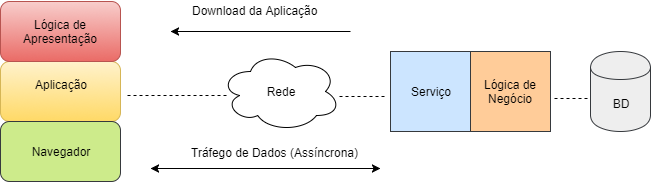
\includegraphics[width=8cm]{Figuras/Cap1/arquiteturaModerna.png}
\caption[]{Observe que toda a lógica de apresentação é feita no lado cliente e o servidor fica somente com a lógica de negócio} 
\end{figure}

\newpage
\section{Rest}

\subsection{Visão Geral}

Representational State Transfer(REST), em português Transferência de Estado Representacional é uma abstração da arquitetura da World Wide Web (Web), é um estilo arquitetural que consiste de um conjunto coordenado de restrições arquiteturais aplicadas a componentes, este estilo foi apresentado e definido por Roy Fielding em uma tese de doutorado PHD.\cite{wikipediaRest}. REST ignora os detalhes das implementações dos componentes e a sintaxe do protocolo, com o objetivo de focar nos papéis dos componentes, as restrições sobre suas interações com os componentes e suas interpretações de dado elementos significativos.  \cite{royFielding}
A ideia é formalizar um conjunto de restrições(constraints) aplicado para elementos dentro de uma arquitetura, e aproveitar de fato todos os recursos oferecidos pelos padrões, como por exemplo Http e Uri.
Segundo \cite{royFielding}, há duas perspectivas comuns em processos de projetos. A primeira é que um projeto começa vazio e a partir das necessidades começa a se construir uma arquitetura de componentes familiares. A segunda é que um projeto começa com necessidades de um sistema como um todo, sem restrições, após isto é identificado e aplicado as restrições aos elementos do sistema. A primeira enfatiza a criatividade e visão ilimitada, a segunda a restrição e a compreensão do contexto. O REST entra no segundo processo com um conjunto incremental de restrições. Vamos ver cada uma das restrições:

\subsection{Cliente Servidor}
A primeira restrição segundo \cite{royFielding}, diz respeito a separação dos papéis e responsabilidades das diferentes parte de um sistema. Por exemplo separar a interface do usuário e servidor back end e aumentar a escalabilidade do sistema.

\subsection{Stateless}
A comunicação do cliente com o servidor deve ser stateless, toda Solicitação que o cliente fizer ao servidor deve conter todas as informações para que esta seja tratada com sucesso e as próximas requisições não devem ter ligações com as anteriores. Segundo \cite{royFielding}, utilizando um modelo de comunicações stateless, sua API passa a ter características como visibilidade, confiabilidade e escalabilidade.

\subsection{Cache}
Um sistema com REST, deve permitir que suas respostas sejam passíveis de cache. A vantagem segundo \cite{royFielding} é que sistemas assim, tem o potencial de eliminar parcialmente ou totalmente algumas interações, melhorando a latência entre o cliente e servidor, e ainda, melhorando a eficiência, a escalabilidade e o desempenho percebido pelo usuário na utilização do sistema.

\subsection{Interface Uniforme}
Uma das características que mais distingue o REST dos outros estilos arquiteturais baseado na web é a sua ênfase na Interface Uniforme entre componentes \cite{royFielding}. Ao se criar um recurso, que utilize por exemplo o protocolo HTTP, deve se levar em consideração a utilização dos seus respectivos métodos de forma correta. Segundo \cite{royFielding}, REST é definido por quatro restrições de interfaces, são elas: Identificação de recursos, manipulação de recursos através de representações, mensagens auto descritivas e hypermedia como o motor da aplicação.

\subsection{Sistema em Camadas}
Permite que uma arquitetura seja composta de camadas hierárquicas ao restringir o comportamento dos componentes, de modo que um componente não possa ver além da camada imediata com a qual ele esteja interagindo\cite{royFielding}.

\subsection{Código sob Demanda}
O código sob demanda permiti adaptar os clientes de acordo com os novos requisitos e funcionalidades. Contudo segundo \cite{royFielding} isso pode reduzir a visibilidade e por isso é uma restrição opcional.

\subsection{Recursos}
A URI é uma das funcionalidades do REST que é utilizar recursos baseado nas especificações da RFC 3986. Nas especificações \cite{rfc3986} diz que um URI (A Uniform Resource Identifier), Identificador de Recurso Uniforme é uma sequência compacta de caracteres que identifica um recurso abstrato ou físico, cada recurso tem um esquema de nomes, que começa com letras e seguido de qualquer combinação de letras, dígitos, mais (+), perído (.), ou hífen (-), deve ser feito com letras minúsculas. Basicamente é utilizado substantivos nos nomes e não verbos, por exemplo, se queremos criar um recurso para veículos, o nome deste seria '/veiculo', sempre um nome e nunca uma ação.

\subsection{Representações e Métodos Http}
A comunicação mais comum entre o cliente e o servidor é feita pelo protocolo HTTP, tudo o que é trocado entre eles são as chamadas representações, ou negociação de conteúdo, cujo seu formato deve suporta a utilização de hypermedia, como JSON, XML, HTML, entre outros listados são considerados modelos de representação. Um exemplo seria um cliente solicitar um recurso cuja sua representação é em formato HTML, ele informa no cabeçalho da solicitação o conteúdo aceitável. Quando o servidor recebe uma solicitação do cliente, ele verifica o conteúdo informado na solicitação deste, se o conteúdo for compatível, ou seja, se houver um dado conhecido e suportado pelo servidor, ele fornecerá este conteúdo com o formato desejado, este é o chamado negociação de conteúdo realizada com sucesso. Para um determinado recurso específico, há um conjunto de métodos que seguem uma semântica de operações. A RFC 7231 escrita por \cite{rfc7231} especifica que este conceito indica o propósito para o qual o cliente fez esse pedido e o que é esperado pelo cliente como um resultado bem sucedido. Abaixo são listados os método utilizados na identificação do recurso pela solicitação da URI informada, de acordo com a especificação da RFC 7231 listadas por \cite{rfc7231}:

\begin{itemize}
\item GET - Obtém uma representação selecionada atual para um recurso de origem.
\item POST - Solicita a criação de recursos no servidor de origem.
\item PUT - Solicita a criação ou modificação no servidor de origem.
\item DELETE - Remove um recurso e sua atual funcionalidade.
\item CONNECT - Solicita que o destinatário estabeleça um túnel para o servidor de origem.
\item OPTIONS - Solicita informações sobre as opções disponíveis de comunicação para o recurso de destino.
\item TRACE - Solicita um remoto loopback(canal de comunicação) de nível de aplicação da mensagem solicitada.
\end{itemize}

Para cada solicitação feita ao servidor utilizando qualquer um dos métodos HTTPs listados acima há uma resposta retornada pelo servidor de destino para o recurso de destino, ou seja, o servidor gera uma resposta para o cliente que solicitou um recurso. Esta resposta é representada por um elemento inteiro de três dígitos chamado de "Response Status Codes" (Códigos de estados da resposta). 

\begin{quote}
"Os clientes HTTP não são obrigados a entender o significado de todos os códigos de estados, embora a compreensão é obviamente desejável. No entanto um cliente deve compreender as classes de qualquer código de estado conforme indicado pelo primeiro dígito, cujo este primeiro dígito define uma classe, os outros dois dígitos não tem qualquer papel de categorização" \cite{rfc7231}.
\end{quote}

Na especificação RFC 7231 citada por \cite{rfc7231} são listados cinco valores para o primeiro dígito: 
\begin{itemize}
\item 1xx (Informativo): A solicitação foi enviada, processo contínuo.
\item 2xx (Bem Sucedido): A solicitação foi recebida com sucesso, entendida e aceita.
\item 3xx (Redirecionamento): Outra ação precisa ser tomada na sequência para completar a solicitação.
\item 4xx (Erro do Cliente): A solicitação contém uma sintaxe ruim ou não pode ser realizada.
\item 5xx (Erro do Servidor): O servidor falhou para realizar uma solicitação válida aparentemente.
\end{itemize}

Segue abaixo uma tabela com um resumo do que cada código representa, citado na especificação RFC 7231:

\begin{table}
\caption{Response Code Status}
\centering
\begin{tabular}{r 1r 2l}
Code & Reason & Defined in \\
\hline 
100	&	Continue                      	&	Section 6.2.1            	\\
101	&	Switching Protocols           	&	Section 6.2.2            	\\
200	&	OK                            	&	Section 6.3.1            	\\
201	&	Created                       	&	Section 6.3.2            	\\
202	&	Accepted                      	&	Section 6.3.3            	\\
203	&	Non-Authoritative Information 	&	Section 6.3.4            	\\
204	&	No Content                    	&	Section 6.3.5            	\\
205	&	Reset Content                 	&	Section 6.3.6            	\\
206	&	Partial Content               	&	Section 4.1 of [RFC7233] 	\\
300	&	Multiple Choices              	&	Section 6.4.1            	\\
301	&	Moved Permanently             	&	Section 6.4.2            	\\
302	&	Found                         	&	Section 6.4.3            	\\
303	&	See Other                     	&	Section 6.4.4            	\\
304	&	Not Modified                  	&	Section 4.1 of [RFC7232] 	\\
305	&	Use Proxy                     	&	Section 6.4.5            	\\
307	&	Temporary Redirect            	&	Section 6.4.7            	\\
400	&	Bad Request                   	&	Section 6.5.1            	\\
401	&	Unauthorized                  	&	Section 3.1 of [RFC7235] 	\\
402	&	Payment Required              	&	Section 6.5.2            	\\
403	&	Forbidden                     	&	Section 6.5.3            	\\
404	&	Not Found                     	&	Section 6.5.4            	\\
405	&	Method Not Allowed            	&	Section 6.5.5        
\end{tabular}
\end{table}

\begin{table}
\caption{Continuação Response Code Status}
\centering
\vspace{0.5cm}
\begin{tabular}{r 1r}
Code & Reason & Defined in \\
\hline 
406	&	Not Acceptable                	&	Section 6.5.6            	\\
407	&	Proxy Authentication Required 	&	Section 3.2 of [RFC7235] 	\\
408	&	Request Timeout               	&	Section 6.5.7            	\\
409	&	Conflict    &	Section 6.5.8 \\
410	&	Gone                          	&	Section 6.5.9            	\\
411	&	Length Required               	&	Section 6.5.10           	\\
412	&	Precondition Failed           	&	Section 4.2 of [RFC7232] 	\\
413	&	Payload Too Large             	&	Section 6.5.11           	\\
414	&	URI Too Long                  	&	Section 6.5.12           	\\
415	&	Unsupported Media Type        	&	Section 6.5.13           	\\
416	&	Range Not Satisfiable         	&	Section 4.4 of [RFC7233] 	\\
417	&	Expectation Failed            	&	Section 6.5.14           	\\
426	&	Upgrade Required              	&	Section 6.5.15           	\\
500	&	Internal Server Error         	&	Section 6.6.1            	\\
501	&	Not Implemented               	&	Section 6.6.2            	\\
502	&	Bad Gateway                   	&	Section 6.6.3            	\\
503	&	Service Unavailable           	&	Section 6.6.4            	\\
504	&	Gateway Timeout               	&	Section 6.6.5            	\\
505	&	HTTP Version Not Supported    	&	Section 6.6.6  

\end{tabular}
\end{table}

\newpage
\section{Angular}

Segundo a documentação do Angular \url{https://angular.io/docs}, este é framework que usa uma plataforma que facilita a criação de aplicativos na web que combina modelos declarativos, injeção de dependência, ferramentas de ponta a ponta e melhores práticas integradas para resolver desafios de desenvolvimento, o Angular capacita desenvolvedores a construir aplicativos que vivem na web, no celular ou na Área de trabalho. A intenção é utilizar esta ferramenta para construir um aplicativo para o lado cliente utilizando HTML ou Javascript ou Typescript que compila para Javascript.

\subsection{Visão Geral da Arquitetura}
Este framework contém várioas bibliotecas, algumas são do próprio núcleo outras são opcionais. A ideia é compor modelos de telas (templates) com HTML, escrever classes de componentes para gerenciar esses modelos depois aplicar lógica de aplicativo em serviços, tudo isto dentro de módulos, mas todos centralizados no componente. Um imagem da arquitetura é exibido abaixo: 

\begin{figure}[!h]
\centering
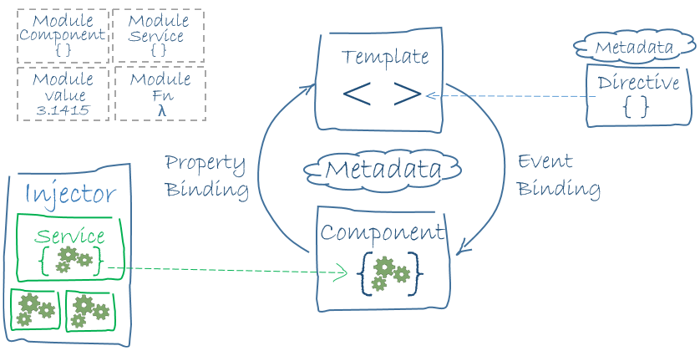
\includegraphics[width=8cm]{Figuras/Cap2/OverviewAngular.png}
\caption[]{Visão geral da arquitetura de uma aplicação em Angular}
\end{figure}

\subsection{Módulos}
A documentação do Angular \url{https://angular.io/docs} explica que aplicativos em Angular são modulares, e contém o seu próprio sistema de modularização chamado de 'NgModules'. A intenção é organizar cada funcionalidade do aplicativo dentro de módulos.
Toda aplicação inicia com um módulo raiz chamado de 'AppModule', para criar um módulo, deve-se criar uma classe e marcá-la com um decorator\footnote{São funcionalidades que modificam classes javascripts} chamado '@NgModule' que contém metadados com propriedades que descrevem um módulo e informa para o Angular como compilar e executar o código deste, as propriedades destes metadados são descritas abaixo:

\begin{itemize}

\item declarations (declarações): as views\footnote{O Angular tem três tipos de views: Componentes, diretivas e pipes(tubos)} que pertencem a um módulo.

\item exports (Exportações): um subconjunto de declarações que devem ser visíveis e utilizáveis no modelo(template) de componente de outros módulos.

\item imports (Importações): Outros módulos cuja as classes exportadas são necessárias por modelos(templates) de componentes declarados deste módulo.

\item providers (Fornecedores): Criadores de serviços que este módulo contribui para uma coleção global de serviços, eles se tornam acessíveis para todas as partes da aplicação.

\item bootstrap: Aplicado somente a view principal da aplicação, chamada de 'root component', que hospeda todas as outras views.   
\end{itemize}

Está é a estrutura de uma módulo raiz da aplicação:

import { NgModule }      from '@angular/core';

import { BrowserModule } from '@angular/platform-browser';

@NgModule({

  imports:      [ BrowserModule ],
  
  providers:    [ Logger ],
  
  declarations: [ AppComponent ],
  
  exports:      [ AppComponent ],
  
  bootstrap:    [ AppComponent ]
  
})

export class AppModule { }

\subsection{Componentes e Modelos}
Na documentação do Angular \url{https://angular.io/docs}, um componente é quem controla um pedaço da tela de uma view. Um modelo ou template\footnote{É um formulário em HTML que informa ao Angular como se tornar(to render) um componente.} é definido com um view de componentes com seus modelos complementares.


\subsection{Metadados}
Metadados dizem ao Angular como processar uma classe, é necessário aplicar um decorator na classe, veja abaixo um exemplo com um decorator '@Component':

@Component({

  selector:    'hero-list',
  
  templateUrl: './hero-list.component.html',
  
  providers:  [ HeroService ]
  
})

export class HeroListComponent implements OnInit {

/* . . . */

}

\subsection{Ligação de Dados}
Ligar os dados ou o mais conhecido data binding é um mecanismo para coordenar partes de um modelo/template com as partes de um componente, na figura acima é exibido quatro formas de declarar um data bindind, cada forma tem uma direção, para o DOM, vindo do DOM, ou em ambas as direções, veja abaixo:

\begin{figure}[!h]
\centering
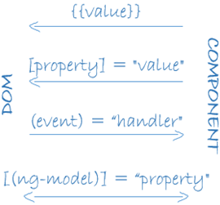
\includegraphics[width=8cm]{Figuras/Cap2/databinding.png}
\caption[]{Formas de declarações de data bindings}
\end{figure}

\subsection{Diretivas}
Uma diretiva é uma classe marcada com um decorator '@Directive', mas o decorator '@Component' já herda essa funcionalidade das diretivas. Quando o Angular renderiza seus templates o DOM é transformado de acordo com as instruções das diretivas. Dois outros tipos de diretivas são: Estrutural e a diretiva de atributos. Eles são utilizadas dentro de tags como propriedade em um HTML, a diretiva estrutural, altera um layout por adição, remoção, substituição de elementos no DOM. A diretiva de atributos, altera uma aparência ou comportamentos de uma elemento.
Exemplo de uma diretiva estrutural e de atributo:

<li *ngFor="let hero of heroes"></li>

<input [(ngModel)]="person.name">


\subsection{Serviços}
Um serviço no Angular é um ampla categoria abrangendo qualquer valor, funções, ou características que a aplicação necessita. É uma classe com um propósito bem definido. Algums exemplos de serviços são: categorias, marca de veículos, logs de um sistema entro outros.

\subsection{Injeção de Dependência}
A Injeção de dependência é a uma maneira de fornecer instâncias de classes com suas dependências totalmente formadas que ela requer. O Angular a utiliza para fornecer novos componentes. 